\chapter{Measuring Team Progress and Adaptation}
\label{ch:agile-evaluation}

Adopting Agile practices represents only the beginning. Teams must continuously evaluate whether their implementation delivers value and where further improvement is possible. Empiricism requires inspection and adaptation based on transparent information \textit{\parencite{schwaber2020scrum}}. Research shows that teams demonstrating responsiveness through frequent releases achieve higher stakeholder satisfaction \textit{(Russo, ASE Lecture 3, 2025)}. This chapter examines how Djøf Trade Union measures their Agile effectiveness and evolves their practices.

\section{Sprint Reviews and Stakeholder Engagement}
\label{sec:sprint-reviews}

Djøf Trade Union established regular sprint reviews to evaluate completed work and gather feedback. After each sprint, they review what they accomplished, whether goals were met, and what can be learned \textbf{(Transcript: 00:06:48--00:07:31)}. These reviews provide structured moments for reflection rather than pushing forward blindly.

Sprint reviews involve stakeholders from the business side. The team invites interested parties to see what they built, and quarterly demos showcase three months of accumulated progress to broader audiences \textbf{(Transcript: 00:20:37--00:21:07)}. This regular demonstration rhythm keeps stakeholders informed without constant interruptions to the development team.

The review process helps the team understand whether their work delivers actual value. When features reach users, the Product Owner and business teams collect feedback and bring it back to development \textbf{(Transcript: 00:21:07--00:21:37)}. This creates a feedback loop where user experience influences future prioritization. Success is not just completing tasks but solving real problems for members and internal users.

\section{Retrospectives and Process Refinement}
\label{sec:retrospectives}

Beyond reviewing product increments, Ahmed's team holds retrospectives to examine their working methods. These sessions focus on how the team collaborates and what obstacles prevent smooth workflow \textbf{(Transcript: 00:07:31--00:07:48)}. Sprint Retrospectives enable teams to reflect on their process and identify improvements for future iterations \textit{(Russo, ASE Lecture 3, 2025)}.

One concrete improvement emerged from retrospective discussions: code reviews were taking too long because colleagues lacked time to examine pull requests promptly \textbf{(Transcript: 00:23:07--00:23:37)}. The team agreed that when someone creates a pull request and announces it in Teams, a reviewer must examine it within four hours \textbf{(Transcript: 00:23:37--00:24:07)}. This simple commitment dramatically improved their development flow.

The team's pragmatic adaptation of Scrum also appears in retrospectives. When a sprint lacks meaningful progress, they sometimes skip the retrospective because there is little to reflect upon \textbf{(Transcript: 00:09:59--00:10:22)}. This flexibility demonstrates their focus on value rather than ceremony for ceremony's sake.

\section{Tracking Metrics and Leadership Support}
\label{sec:tracking-metrics}

Djøf Trade Union tracks concrete indicators of progress. They measure how many tasks complete per sprint, providing insight into team capacity \textbf{(Transcript: 00:21:52--00:22:22)}. They also track lead time from when a task starts until it deploys to production, highlighting bottlenecks in their process.

Quality metrics complement velocity tracking. The team monitors how many bugs surface during development versus how many escape to production \textbf{(Transcript: 00:22:22--00:22:52)}. This indicates whether their testing catches issues before users encounter them. Quality assurance practices and clear Definition of Done criteria help teams maintain consistent standards \textit{(Russo, ASE Lecture 5, 2025)}. High production bug rates signal problems with testing or code review processes.

The organization's measurement approach remains practical rather than exhaustive. They gather enough data to spot trends and identify problems without drowning in metrics. The goal is actionable insight, not comprehensive dashboards. When code review delays appeared in their data and team discussions, they took concrete action rather than simply documenting the problem.

\begin{figure}[h]
\centering
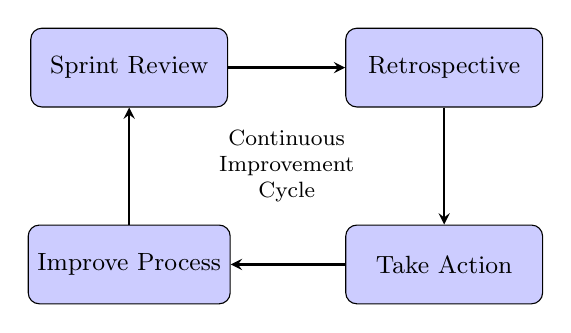
\begin{tikzpicture}
    % Define styles
    \tikzstyle{process} = [rectangle, rounded corners, minimum width=2.5cm, minimum height=1cm,
                          text centered, draw=black, fill=blue!20, font=\small]
    \tikzstyle{arrow} = [thick,->,>=stealth]

    % Nodes positioned absolutely
    \node[process] (review) at (0,0) {Sprint Review};
    \node[process] (retro) at (4,0) {Retrospective};
    \node[process] (action) at (4,-2.5) {Take Action};
    \node[process] (improve) at (0,-2.5) {Improve Process};

    % Arrows
    \draw[arrow] (review) -- (retro);
    \draw[arrow] (retro) -- (action);
    \draw[arrow] (action) -- (improve);
    \draw[arrow] (improve) -- (review);

    % Center label
    \node[font=\footnotesize, text width=2cm, align=center] at (2,-1.25) {Continuous\\Improvement\\Cycle};
\end{tikzpicture}
\caption{Continuous improvement cycle through regular sprint reviews and retrospectives}
\label{fig:improvement-cycle}
\end{figure}


The combination of sprint reviews, retrospectives, and lightweight metrics creates continuous improvement. The organization demonstrates that Agile evaluation doesn't require sophisticated tools or extensive data collection. Regular inspection of both product and process, coupled with willingness to adapt when issues surface, drives meaningful improvement over time.

Management support reinforces this learning orientation \textbf{(Transcript: 00:24:22--00:25:22)}, allowing them to invest time in addressing problems rather than only delivering features. Leadership provides resources for skill development and respects process boundaries. When they request tools or training, management evaluates requests seriously. This support creates psychological safety where teams can acknowledge problems without fear, enabling honest retrospectives and genuine improvement.
